% This file was created with tikzplotlib v0.10.1.
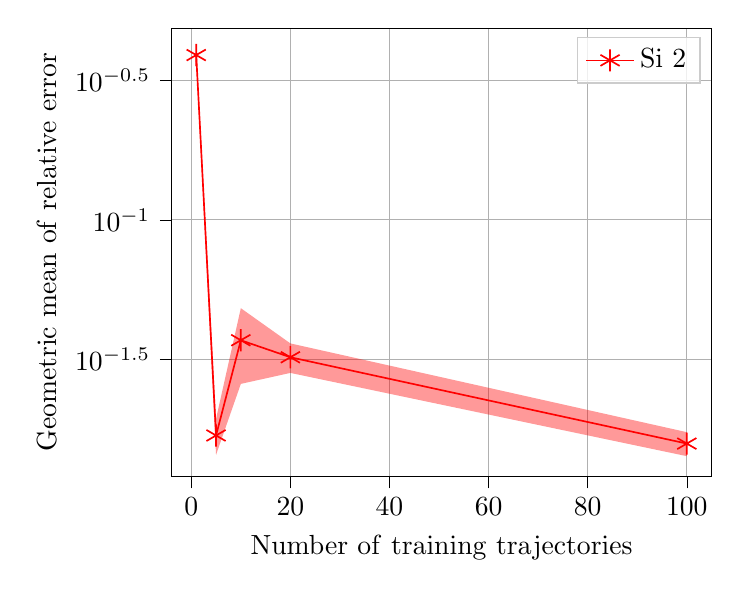
\begin{tikzpicture}

\definecolor{darkgray176}{RGB}{176,176,176}
\definecolor{lightgray204}{RGB}{204,204,204}

\begin{axis}[
legend cell align={left},
legend style={fill opacity=0.8, draw opacity=1, text opacity=1, draw=lightgray204},
log basis y={10},
tick align=outside,
tick pos=left,
x grid style={darkgray176},
xlabel={\(\displaystyle \mathrm{Number \ of \ training \ trajectories }\)},
xmajorgrids,
xmin=-3.95, xmax=104.95,
xtick style={color=black},
y grid style={darkgray176},
ylabel={\(\displaystyle \mathrm{Geometric \ mean \ of \ relative \ error }\)},
ymajorgrids,
ymin=0.0120590510734795, ymax=0.485384509596417,
ymode=log,
ytick style={color=black}
]
\path [fill=red, fill opacity=0.4, semithick]
(axis cs:1,0.410337960086159)
--(axis cs:1,0.367981594058864)
--(axis cs:5,0.0144215000794806)
--(axis cs:10,0.0258840064863564)
--(axis cs:20,0.028333380200394)
--(axis cs:100,0.014264526221922)
--(axis cs:100,0.0173867832524469)
--(axis cs:100,0.0173867832524469)
--(axis cs:20,0.0361384012520683)
--(axis cs:10,0.0483010038838213)
--(axis cs:5,0.0194167039826465)
--(axis cs:1,0.410337960086159)
--cycle;

\addplot [semithick, red, mark=asterisk, mark size=4, mark options={solid}]
table {%
1 0.389159768819809
5 0.0169191025197506
10 0.0370925106108189
20 0.0322358869016171
100 0.0158256553113461
};
\addlegendentry{Si 2}
\end{axis}

\end{tikzpicture}
